\section{Results}
We evaluated the effect of imputation, using only the training set, by down-sampling the three alleles with the most training data to a range of simulated training set sizes and testing on the remaining data (Figure ~\ref{fig:imputecomparison}). We find that imputation gives a modest improvement up to approximately 100 training samples. With more training data there is no benefit to imputation. The results are similar for the two other performance metrics (not shown).

% The figure doesn't show up in the preview but does show up if you export to pdf.
\begin{figure}[hb]
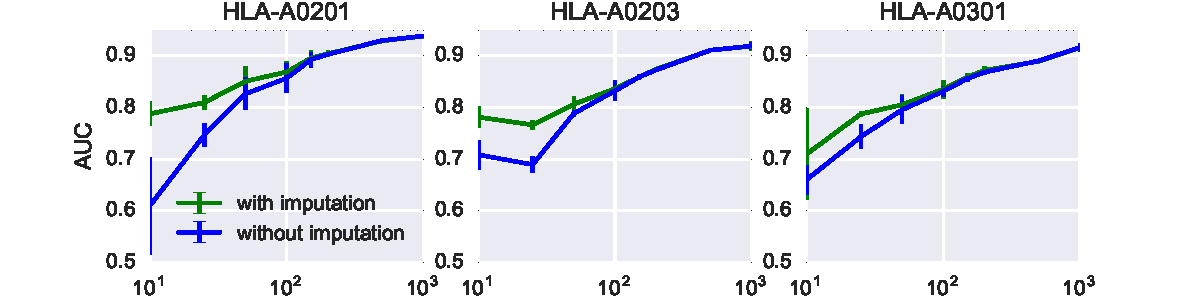
\includegraphics{figures/impute_comparison.pdf}
\caption{\label{fig:imputecomparison} MHCFlurry AUC on down-sampled training data with and without imputation}
\end{figure}

We compared the performance of two MHCFlurry-based models, ``mhcflurry ensemble'' and ``mhcflurry single,'' against netMHC, netMHCpan, and smmpmbec on the blind test data. The ``mhcflurry single'' model is one predictor with the architecture described previously. The ``MHCFlurry ensemble'' model is an ensemble of 10 predictors, each identical to the single predictor with different random initial weights.

The MHCFlurry ensemble predictor is competitive with netMHC, but slightly worse than netMHCpan, especially on alleles with little training data. For 6 of the 7 alleles with fewer than 500 training examples, MHCFlurry underperforms (in terms of AUC) both netMHC and netMHCpan. On the 44 alleles with at least 500 observations, however, the MHCFlurry ensemble slightly outperforms the other models. The ensemble predictor reliably outperforms the single model, as expected.

The BD2009 / BLIND train and test datasets do not contain any alleles with fewer than 200 training observations. Since imputation only seems to help for alleles with fewer than 100 observations, this benchmark may not benefit from the imputation approach.

In conclusion, the MHCFlurry ensemble shows state of the art performance on alleles with at least 500 training examples but slightly worse performance than netMHC and netMHCpan on alleles with fewer observations. Imputing training data shows promise in cross-validation as a way to improve performance on alleles with few observations, but only seems to help for very small training sizes ($\leq 100$), not the alleles in the intermediate regime of $200-500$ present in our benchmark data. Further work is required to assess the accuracy of MHCFlurry and other predictors on alleles with very few training examples and improve MHCFlurry's performance in the intermediate regime.


% These are generated in the 'paper plots' notebook; do not edit by hand.


\begin{table}[h]
\centering
\begin{tabular}{llll}
\toprule
{} &              AUC &      $F_1$ score & Kendall's $\tau$ \\
\midrule
mhcflurry ensemble &           0.9325 &           0.7847 &  \textbf{0.5865} \\
mhcflurry single   &           0.9313 &           0.7831 &           0.5843 \\
netmhc             &           0.9323 &  \textbf{0.8072} &           0.5863 \\
netmhcpan          &  \textbf{0.9326} &           0.7996 &           0.5814 \\
smmpmbec cpp       &           0.9213 &           0.7903 &           0.5649 \\
\bottomrule
\end{tabular}

\caption{Performance on BLIND}
\label{tab:measurementweighted}
\end{table}